%!TEX root = ../Tibt.tex

\exercise{3.17}

\seecode

The notebook for this exercise reproduces the results for the \texttt{prostate}
dataset before repeating the analysis on the \texttt{spam} dataset.

A few notes:

\begin{itemize}
    \item I interpreted the exercise as requiring one to perform
      \textit{regression} on the binary response variable.
    \item I found some significant deviations from the values
      of Table 3.3 in the text, even for simple OLS - it isn't clear
      to me where such deviations come from.
    \item The cross-validated parameter values also seem to differ, for
      some model families, from the ones implicitly used in Table 3.3.
      This is less surprising: the fold indices used by the authors
      are not known.
    \item In the \texttt{spam} case, which has $57$ predictors, exhaustive
      best subset regression is unfeasible, so I dropped the model
      family from the study.
    \item \texttt{scikit-learn} was used where possible, only providing
      an implementation where the regularization was parametrized in
      a \texttt{scikit}-friendly way in the book.
\end{itemize}

\begin{figure}
\begin{minipage}{\textwidth}
    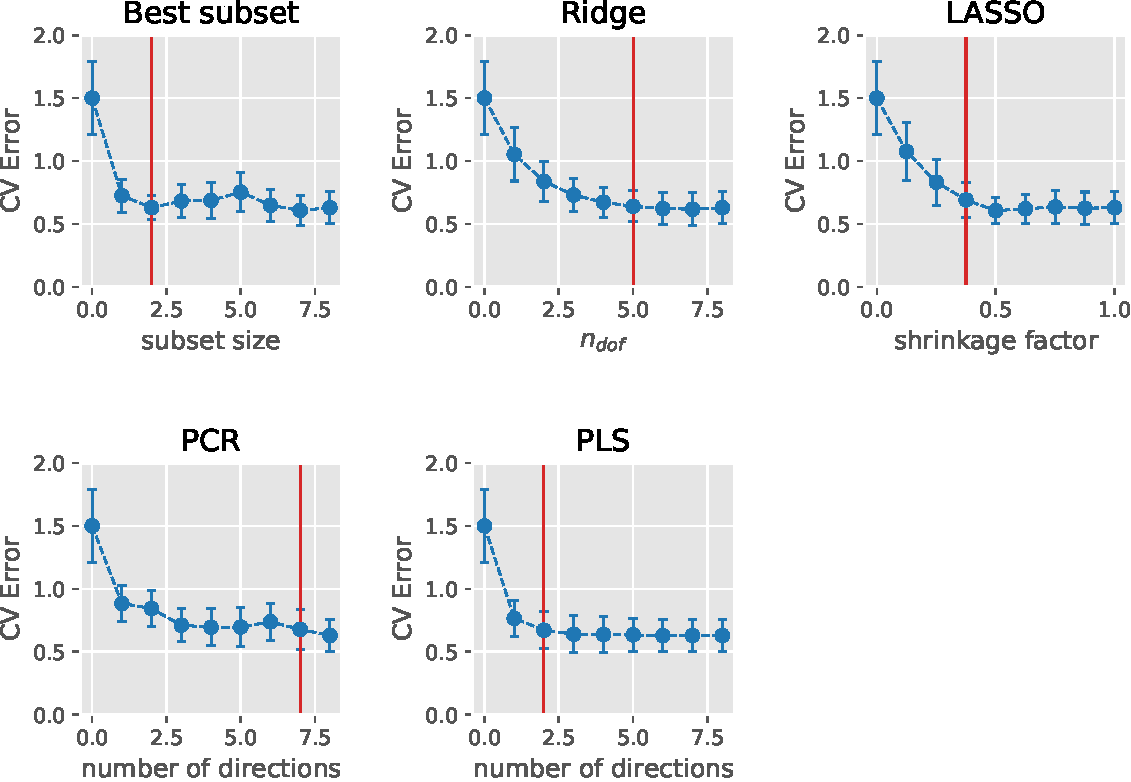
\includegraphics[width=\textwidth]{E3p17_A.pdf}
\end{minipage}\vspace{1cm}\\

\begin{minipage}{\textwidth}
    \centering
    \begin{tabular}{lrrrrrr}
        \toprule
        Term &     OLS & Best subset &   Ridge &  LASSO &     PCR &     PLS \\
        \midrule
        Intercept      &   2.452 &       2.452 &   2.452 &  2.452 &   2.452 &   2.452 \\
        \texttt{lcavol}         &   0.711 &       0.774 &   0.433 &  0.558 &   0.566 &   0.436 \\
        \texttt{lweight}        &   0.290 &       0.349 &   0.252 &  0.187 &   0.321 &   0.360 \\
        \texttt{age}            &  -0.141 &             &  -0.046 &        &  -0.153 &  -0.021 \\
        \texttt{lbph}           &   0.210 &             &   0.168 &  0.002 &   0.214 &   0.243 \\
        \texttt{svi}            &   0.307 &             &   0.234 &  0.094 &   0.320 &   0.259 \\
        \texttt{lcp}            &  -0.287 &             &   0.003 &        &  -0.050 &   0.086 \\
        \texttt{gleason}        &  -0.021 &             &   0.042 &        &   0.227 &   0.006 \\
        \texttt{pgg45}          &   0.275 &             &   0.134 &        &  -0.063 &   0.084 \\
        \midrule
        Test Error     &   0.521 &       0.492 &   0.492 &  0.479 &   0.448 &   0.536 \\
        Test Error Std &   0.179 &       0.143 &   0.162 &  0.164 &   0.104 &   0.149 \\
        \bottomrule
    \end{tabular}
\end{minipage}
\caption{\texttt{prostate} dataset: reproducing Figure 3.7 and Table 3.3}
\end{figure}

\begin{figure}
    \begin{minipage}{\textwidth}
        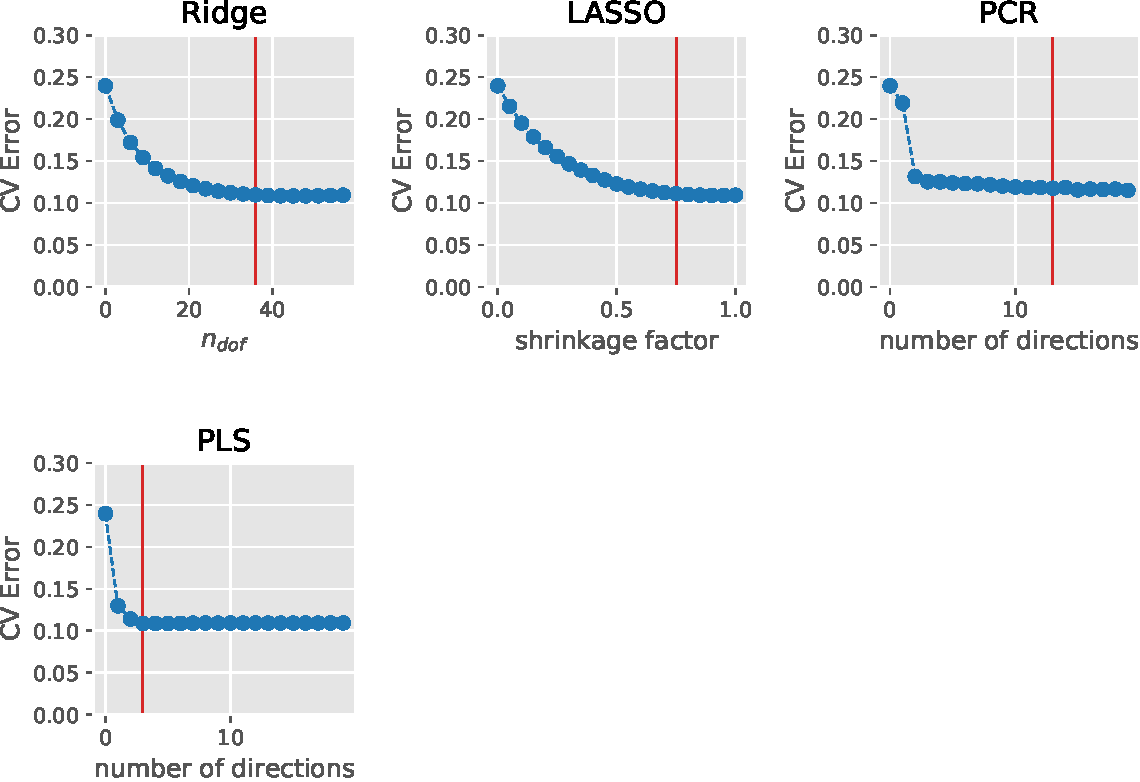
\includegraphics[width=\textwidth]{E3p17_B.pdf}
    \end{minipage}\vspace{1cm}\\
    
    \begin{minipage}{\textwidth}
        \centering
        \begin{tabular}{llllll}
            \toprule
            {} &    OLS &  Ridge &  LASSO &    PCR &    PLS \\
            \midrule
            Test Error     &  0.121 &  0.117 &  0.122 &  0.126 &  0.123 \\
            Test Error Std &  0.007 &  0.005 &  0.007 &  0.005 &  0.008 \\
            \bottomrule
        \end{tabular}
    \end{minipage}
    \caption{\texttt{spam} dataset results.}
\end{figure}


